\documentclass[12pt,a4paper]{article}
\usepackage[english]{babel}
\usepackage[T1]{fontenc}
\usepackage{graphicx}
\usepackage{hyperref}
\usepackage[utf8]{inputenc}
\usepackage{parskip}
\usepackage{url}

\title{Program Design and Data Structures, 1DL201 \\
	Uppsala University - 2018 Spring \\
	\textbf{Checkers in Haskell}}
\author{\textit{Daniel Jönsson, Madelene Alanenpää, Henrik Alfken(Schulze)}}
\date{\today, PKD 2017 - 2018}

\begin{document}
\maketitle
\newpage
\tableofcontents
\newpage

\section{Introduction}
After some discussions we decided to implement the game checkers in Haskell. 
``Checkers'' is its  name in US English -- it is known as ``draughts'' in British 
English.
\footnote{\href{https://en.wikipedia.org/wiki/Draughts}
	{https://en.wikipedia.org/wiki/Draughts}}
Our program lets two users play checkers in Haskell against each other. 

Checkers is an old game that can be played on a chess board or on a bigger board. The 
rules can vary quite alot in checkers -- the following description includes some common 
assumptions. All the 12 pieces on each side of the board stand on the dark squares in 
the first 3 rows when the game starts. 

Figure~\ref{fig1} shows an example of a starting board for checkers.
\begin{figure}[htp]
\centering
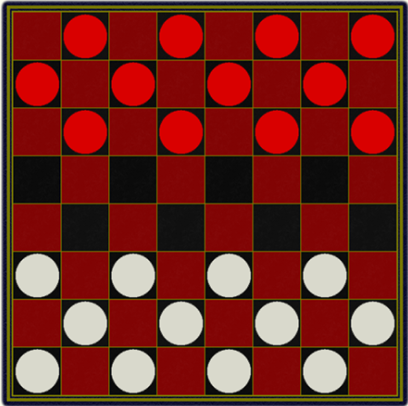
\includegraphics[width= 0.3\textwidth]{Startboarexample.PNG}
\caption{The starting board in an 8x8 checkers.}
\label{fig1}
\end{figure}

In checkers pieces always move diagonally so they will stay on the black squares during 
the whole game. A piece making a non-capturing move (not involving a jump) may move only 
one square in a forward direction.
\footnote{Some versions of the rules allow the pawns to move backwards as well.}
A piece making a capturing move (a jump) stands next to an opponent and leaps over the 
opponent and lands in a straight diagonal line on the other side. The jump can only be 
made if the square after the opponent is empty, so no more than one piece may be 
captured in a single jump. Multiple jumps with one piece should be made if that is 
possible during a single turn. The pieces can jump in both directions when capturing 
opponents.

When a piece is captured, it is removed from the board. If a player can make a capture, 
there is no option; the jump must be made. If captures are available for several pieces, 
the player is free to jump with whichever he or she prefers. When a piece reaches the 
furthest row from the player who controls that piece, it is crowned and becomes a king. 
A king has more freedom and can move several steps in a diagonal line if the line is 
free. When a king makes a jump, it can make it if the space behind the opponent is free 
even if the king is not standing next to that piece.

\section{Summary}
So, what did we accomplish with our work? 

We managed to make a fully functional game in Haskell where it is possible for two 
human players to play checkers. The game follows the rules of checkers as described 
in the introduction with some small exceptions that are described in section 5. 

We have chosen to implement it on a board with 8*8 squares.  Pieces are put out 
diagonally on the first three lines of the board and from here they can only move  
diagonally. When the game starts it is only possible for the red player to move, then 
the players take turns. Pieces can only move one step unless they have the possibility 
to make one or several jumps.
They can’t jump outside the board and a piece will be removed once it has been jumped 
over. If a piece have made a jump and can make another one it must do so or take another 
step. When a piece moves all the way to the "end" of the board it will be transformed 
to a king. A player loses the game when he/she has no more pieces left on the board.

The game prints out a new updated board after every move. Our code will check if a move 
is valid so it is not possible to make a move that is not allowed.

\section{Usage of Program}
To start our program you first need a Haskellplatform with GHCI. This you can download at 
\href{https://www.haskell.org/platform/ }{https://www.haskell.org/platform/ }for Windows, 
Linux and Mac OS X. When the installation is finished in Windows start WinGHCi and load 
\texttt{checkers.hs}. In Mac OS X run the installer, 
follow the instructions and then open Checkers.hs. For Linux follow the instructions on 
the webpage and then open Checkers.hs.
When you have loaded Checkers.hs write main and press enter. Now you will get a starting
board as you can see in Figure~\ref{fig2}. From here you can start to play. 		

\begin{figure}[htp]
\centering
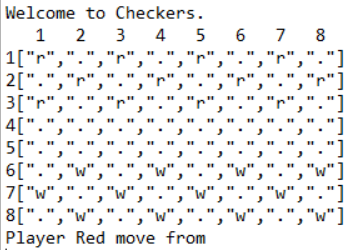
\includegraphics[width= 0.4\textwidth]{start.PNG}
\caption{Welcome to Checkers}
\label{fig2}
\end{figure}

To start you write a tuple with two numbers that represents from where you want to move and press enter. Then you write a new tuple representing to where you want to move and press enter again. The first number in the tuple represents the row and the second represents the column. Look at example below.


Player Red move from

(3,1)

Player Red move to

(4,2)

Player Red moves from  (3,1)  to  (4,2)

Now you will get an updated board with the move applied as you can see in Figure~\ref{fig3},
\begin{figure}[htp]
\centering
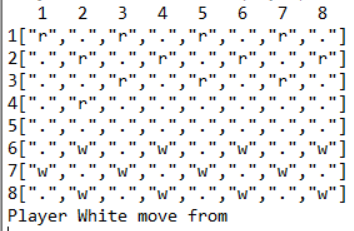
\includegraphics[width= 0.4\textwidth]{firstmove.PNG}
\caption{A Move}
\label{fig3}
\end{figure}

After that it will be whites turn and like this it continues. 
\newpage
To jump over another player you write your "starting coordinates" as usual and the "move to coordinates" behind the player to jump. The board will then be updated with your piece on the new position and the piece you jumped will be removed. If you have possibility to make a jump with more than one piece you can choose which piece you want to jump with. A jump can look something like Figure~\ref{fig4} where red jumps from position (4,2) to (6,4).

\begin{figure}[htp]
\centering
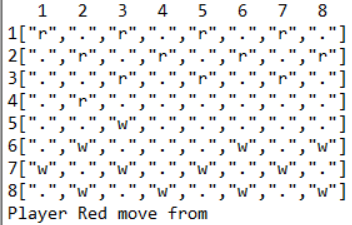
\includegraphics[width= 0.4\textwidth]{jump1.PNG}
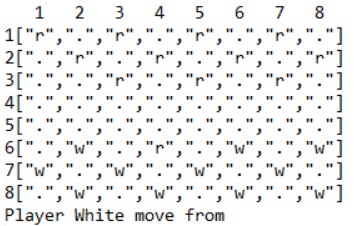
\includegraphics[width= 0.4\textwidth]{jump2.PNG}
\caption{Jump}
\label{fig4}
\end{figure}


If you have possibility to make several jumps with one piece you have to do that once you have made the first jump. You make the first jump as usual and a new board will be printed. Now you can make another jump and you can not move another piece. You make the next jump in the same way as any other jump. In the pictures Figure~\ref{fig5} you can see how the red player makes multiple jumps from position (4,4) to (6,6) and from (6,6) to (8,8) before it is whites turn.


\begin{figure}[htp]
\centering
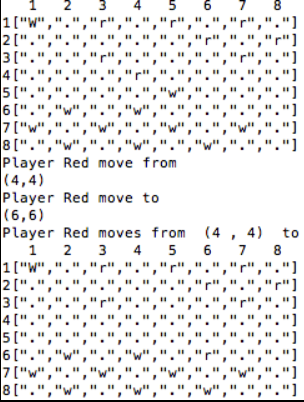
\includegraphics[width= 0.4\textwidth]{mj1.PNG}
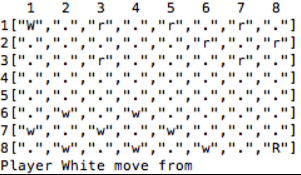
\includegraphics[width= 0.4\textwidth]{mj2.PNG}
\caption{Double Jump}
\label{fig5}
\end{figure}



If a player moves over the board to the other side it will be upgraded to a king and that will be represented with a capital r or a capital w, see Figure~\ref{fig6} where a red piece have moved to the other side, position (8,6).


\begin{figure}[htp]
\centering
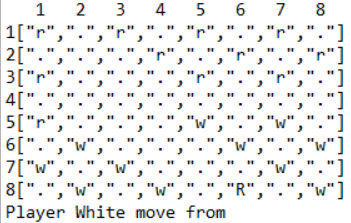
\includegraphics[width= 0.4\textwidth]{queen.PNG}
\caption{King}
\label{fig6}
\end{figure}

A player wins when the opponent have no more pieces on the board and then you can choose if you want to quit or continue. The end board can look like Figure~\ref{fig7}.

\begin{figure}[htp]
\centering
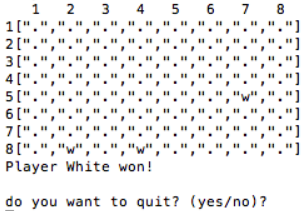
\includegraphics[width= 0.4\textwidth]{victory.PNG}
\caption{Winner}
\label{fig7}
\end{figure}


If you write a move that is invalid you will get a message that says something like this.

\textit{"Player Red moves from (3 , 1) to (1 , 4)
Invalid Move. You can only move your own pieces and move diagonally"}

\textit{"Player Red move from"}

If you write your move in the wrong format you will get a message that says 

\textit{"Invalid input. Correct format: (row,column)"}




\section{Program Documentation}
\subsection{Description of data structures}
The data types on the next page are the ones we have defined and use for our checkers game in Haskell. As described earlier in the report the pieces in Checkers are either kings or a pawns that are red or white so we needed some data types that could help us represent this on our board.\\\\
\textbf{data Player = Player Color Type}

\textbf{data Color = Red | White}

\textbf{data Rank = Normal | King}

Since we made our empty board as a list of 64 ".", we didn't need to have data types for representing "." on the board. In the code we use our data types in functions that reads and shows our Players, see Figure~\ref{fig8}. 

\begin{figure}[htp]
\centering
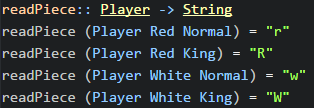
\includegraphics[width= 0.4\textwidth]{read.PNG}
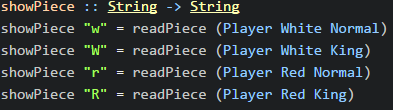
\includegraphics[width= 0.5\textwidth]{show.PNG}
\caption{readPiece and showPiece}
\label{fig8}
\end{figure}

 

We use read- and showPiece in different funtions in our code like in insertPlayer where we use readPiece.

\subsection{Description of algorithms and functions}
\subsubsection{main}
\textbf{Description} \\\\
Generates the starting board for the players and prints it out in the terminal.
It also displays the message "Welcome to Checkers"\\\\
\subsubsection{Printboard}

\textbf{Description}\\\\
Printboard takes a gamestate as argument and returns IO (). It Prints out the board the way it looks at the moment. The argument that printboard takes is patternmatched to (x:y:z:q:a:b:c:d). 

\textbf{Step By Step}

1) Uses putStrln to print 	1   2   3   4   5   6   7   8\\
2) --------""------------ 1 followed by the first row in the board\\
3) --------""------------ 2 followed by the second row in the board\\
4) --------""------------ 3 followed by the third row in the board\\
5) --------""------------ 4 followed by the fourth row in the board\\
6) --------""------------ 5 followed by the fifth row in the board\\
7) --------""------------ 6 followed by the sixth row in the board\\
8) --------""------------ 7 followed by the seventh row in the board\\
9) --------""------------ 8 followed by the eighth row in the board \\\\

\subsubsection{Victory}

\textbf{Description}

victoryRed and victoryWhite takes GameState as argument and returns a Bool. victoryRed checks if there are white players in Gamestate and returns a Bool, that returns True if there aren't any white pieces left and False otherwise. victoryWhite does the same but for red players. Play calls the Victoryfunctions after every move in the game and if VictoryRed or VictoryWhite is True it will put the String "Player Red won!" or "Player white won!"\\
\textbf{Step By Step}

The victory functions concat GameState to one list and are then using victoryAuxRed and victoryAuxWhite to check for a Bool value. The victoryAuxfunctions takes a list as argument and returns a Bool.

1) victoryAux- checks if the list is empty and returns True if that is the case, this is the base case. \\\\
2) If it's not an empty list victoryAuxRed checks if the head (y) of the list (y:ys), y == "w" || == "W". VictoryAuxWhite does the same but with red pieces.\\\\
3) If the second step returns False the victuryAux functions continues with the tail (ys) of the list.\\\\
4) If the victoryAuxfuntions returns true it stops and the functions play will print "Player Red won!" or "Player white won!"


{\subsubsection{play gameState}}
\textbf{Description}\\\\
It generates new gamestates from
the moves entered by player red and player white. It also checks victory conditions.\\\\
\textbf{Step By Step}
\\\\
1) It starts with generating a new gamestate
from the function {\textbf{\small{playerMoveRed gameState}}}.\\\\
2) If victory is achieved for player red
then it displays the message "Player Red won! and runs the function {\textbf{\small{quitPlease}}}, which asks if they want to quit the game or not.\\\\
3) If victory is not achieved for player red it generates a new gamestate from player white from the function {\textbf{\small{playerMoveWhite newGameState}}}.\\\\
4) From this newer gamestate, if victory conditions are met for player white, it shows
the message "Player White won! and runs the function {\textbf{\small{quitPlease}}}.\\\\
5) If victory conditions are not met for player white it loops back to the beginning of {\textbf{\small{play gameState}}}.\\\\

{\subsubsection{validMoveRed and validMoveWhite}}
\textbf{Description}
\\\\They check if the input gotten from the players are valid, the input being a position the player want to move from and a position the player want to move to, and if valid it returns True and otherwise False. The positions are in the form (row number, column number). Both functions are similar except for some minor differences. The auxillary functions called by validMoveRed always have the name red in it, and the auxillary functions called by validMoveWhite always have white in them as well. ValidMoveRed checks the input for player red and validMoveWhite checks the input for player white.\\\\
\textbf{Step By Step}\\\\
1) It starts with adding positions to the gameState and running the function concat on the gameState, making it a list with positions. ValidMoveRed calls {\textbf{\small{validMoveAuxRed}}} and
validMoveWhite calls {\textbf{\small{validMoveAuxWhite}}}.
\\\\
2) Both Aux functions runs the function {\textbf{\small{findPosition}}} on the list to find out how the board looks around the position the player want to move from. It saves these as variables to be used in 
{\textbf{\small{validMoveAuxAuxRed}}} and in \\
{\textbf{\small{validMoveAuxAuxWhite}}}.
\\\\
3) These two AuxAux functions checks if the two positions entered by players are in the form of a "jump"" or a "step", a jump being two steps away diagonally from the position you want to move from and a step being one step away diagonally. If the player red wants to do a jump validMoveAuxAuxRed calls {\textbf{\small{validJumpRed}}}.
If the player white wants to do a jump validMoveAuxAuxWhite calls {\textbf{\small{validJumpWhite}}}. If the player want to take a step
both validMoveAuxAuxRed and validMoveAuxAuxWhite call the function
{\textbf{\small{validMoveOneStep}}}.\\\\
4) ValidJumpRed checks what kind of piece is around where you want to move from. If there is a white piece one step diagonally from you and an empty space two steps diagonally from you, the jump is considered valid. 
ValidJumpWhite works the same way, except it checks if there is a red piece instead.
ValidMoveOneStep works basically the same but only cares that there is a empty space one step diagonally from where you want to move from and only then is it considered valid.
If any of these is valid it returns as True,
otherwise False. 
\\\\


{\subsubsection{playMove}}
\textbf{Description}\\\\If the positions, where the player have entered where to move from and move to, are valid, playMove is called. 
It generates a new gameState where the piece is moved from a position, to another position.\\\\
\textbf{Step By Step}\\\\
1) It starts with adding positions to the gamestate, using concat on it effectively making it a list with positions. It then calls {\textbf{\small{playMoveAux}}}.
\\\\
2) PlayMoveAux saves the positions one step diagonally from the move from position and also saves what is on that position as a variable. With these positions and the list with positions, it calls the function {\textbf{\small{makeaMove}}}.\\\\
3) MakeaMove looks at the position you wanted to move from and the position you wanted to move to. If the difference is (+-2,+-2) it deletes the empty space and then inserts, using the {\textbf{\small{insertAt}}} function the piece you wanted to move two steps diagonally from where that piece were. It does the same thing to the enemy piece the other piece jumped over but in reverse. It deletes the enemy piece and inserts an empty space. It also does this in the move from position, deleting the moved piece and inserting an empty space. 
If the difference is (+1,+1) it deletes the empty space and then inserts the piece you wanted to move one steps diagonally from where that piece were.  It also does this in the move from position, deleting the moved piece and inserting an empty space. The returned value is then an updated list with positions.\\\\
4) The updated list with positions will be returned to playMove where it will delete the positions and make a gamestate from the list.\\\\

{\subsubsection{doubleMoveRed and doubleMoveWhite}}
\textbf{Description}\\\\ DoubleMoveRed and DoubleMoveWhite comes into play after the first jump is made by the player red respectively player white. It forces the player to use the same piece it jumped with to move again.\\\\
\textbf{Step By Step}\\\\
1) It starts with forcing the player to move from the jumped to position and then asks the player for a new position to move to. Both moves are checked by the function {\textbf{\small{readMove}}}, making sure that the input is in the form of (Int,Int). Otherwise a message will be printed out, the message being Invalid input. Correct format: (row,column).\\\\
2) Both moves are printed out in the terminal for the player to see by the {\textbf{\small{printmove}}} function. \\\\
3) The positions entered by the players are checked if they are valid by the functions {\textbf{\small{validplaceWhite}}} and {\textbf{\small{validMoveWhite}}} for player white and {\textbf{\small{validMoveRed}}} and {\textbf{\small{validplaceRed}}} for player red. If the positions enter are not valid a message will be printed out, the message being Invalid Position. You can only move your own pieces and move diagonally.\\\\
4) If the positions entered are valid, the moves will be entered into a new gamestate generated by {\textbf{\small{playMove}}}. In doubleMoveWhite this gameState is printed out, but not in doubleMoveRed.\\\\
5) The next functions called are {\textbf{\small{checkIfCanMakeKingWhite}}} for doubleMoveWhite and {\textbf{\small{checkIfCanMakeKingRed}}}   for doubleMoveRed. These upgrades the piece to a King if certain conditions are met and then prints a new gamestate for the players to see via the function {\textbf{\small{makeKingWhite}}} for player white and {\textbf{\small{makeKingRed}}} for player red. It also returns the gamestate, effectively ending the players turn.\\\\
6) If checkifCanMakeKingWhite and checkIfCanMakeKingRed return False then 
doubleMoveRed prints the actual gameState, doubleMoveWhite don't print anything. After that {\textbf{\small{checkPositionRed}}} for doubleMoveRed and {\textbf{\small{checkPositionWhite}}} for doubleMoveWhite looks up if another jump can be made and if so loops back to the beginning of doubleMoveRed and doubleMoveWhite. 
Otherwise it returns the gamestate as it is.
\\\\
{\subsubsection{playerMoveWhite and playerMoveRed}}
\textbf{Description}\\\\
PlayerMoveWhite is the function for player white and playerMoveRed is the function for player red. They check if the input are valid and if so generates a new gamestate with the input. Note that both functions are called seperately but they are similar enough that they can be in the same function description. \\\\
\textbf{Step By Step}\\\\
1) A message is displayed for the player. 
Player white gets Player White move from and Player Red gets Player Red move from. 
\\\\
2) The player are asked for input where they enter were they wish to move from. {\textbf{\small{readMove}}} is called upon the input and ensures that the input is in the correct format.om.  
{\textbf{\small{readMove}}} is called upon the input and ensures that the input is in the correct format.\\\\
3) The player are asked for input where they enter were they wish to move to. 
A message is displayed for the player. 
Player white gets Player White move to and Player Red gets Player Red move to.{\textbf{\small{playerMoveWhite newGameState}}}.\\\\
4) {\textbf{\small{printmove}}} prints out how the player chose to move.\\\\
5) The positions entered by the players are checked if they are valid by the functions {\textbf{\small{validplaceWhite}}} and {\textbf{\small{validMoveWhite}}} for player white and {\textbf{\small{validMoveRed}}} and {\textbf{\small{validplaceRed}}} for player red. If the positions enter are not valid a message will be printed out, the message being Invalid Position. You can only move your own pieces and move diagonally.\\\\
6) If the positions entered are valid, the moves will be entered into a new gamestate generated by {\textbf{\small{playMove}}}.\\\\
7) The next functions called are {\textbf{\small{checkIfCanMakeKingWhite}}} for playerMoveWhite and {\textbf{\small{checkIfCanMakeKingRed}}}   for playerMoveRed. These upgrades the piece to a King if certain conditions are met and then prints a new gamestate for the players to see via the function {\textbf{\small{makeKingWhite}}} for player white and {\textbf{\small{makeKingRed}}} for player red. It also returns the gamestate, effectively ending the players turn.\\\\
8) If {\textbf{\small{checkIfCanMakeKingWhite}}} and {\textbf{\small{checkIfCanMakeKingRed}}} return False then 
playerMoveRed prints the actual gameState, playerMoveWhite don't print anything. After that {\textbf{\small{checkPositionRed}}} for playerMoveRed and {\textbf{\small{checkPositionWhite}}} for playerMoveWhite looks up if another jump can be made and if so \\
a) for playerMoveWhite prints the gamestate and 
calls the function {\textbf{\small{doubleMoveWhite}}} which allows the player to make a second jump.\\
b) for playerMoveRed it calls the function 
{\textbf{\small{doubleMoveRed}}} which allows the player to make a second jump.\\\\ 
9) Otherwise it another jump can't be made it returns the gamestate as it is.

{\subsubsection{checkPositionRed and checkPositionWhite}}
\textbf{Description}\\\\
Checks if another jump can be made for player red or player white, returns True if a jump can be made and otherwise False. CheckPositionRed is used by player Red and checkPositionWhite is used by player White. \\\\
\textbf{Step By Step}\\\\
1) Both functions start with checking that the input entered by the player indicate that a jump has already been made. That means that a piece has been moved two steps diagonally in the allowed directions. If it has been moved two steps then positions is added to the gamestate, concat is used on it to make it a list with positions and {\textbf{\small{checkPositionsAuxRed}}} is called by checkPositionRed and {\textbf{\small{checkPositionsAuxWhite}}}is called by checkPositionWhite. \\\\
2) Both auxillary functions checks around the piece we want to move is standing and stores, up to two steps diagonally, positions and if it's empty at the position or not. CheckPositionAuxWhite calls {\textbf{\small{checkPositionsAuxAuxWhite}}}
and checkPositionAuxRed calls {\textbf{\small{checkPositionsAuxAuxRed}}}\\\\
3) CheckPositionsAuxAuxWhite looks around the piece and considers a jump possible if a red piece is one step diagonally from the white piece, and there is a empty space two steps away diagonally from the white piece.\\
CheckPositionsAuxAuxRed looks around the piece and considers a jump possible if a white piece is one step diagonally from the red piece, and there is a empty space two steps away diagonally from the red piece.
\\\\
{\subsubsection {makeKingRed and makeKingWhite}}
\textbf{Description}\\\\
Upgrades the piece to a King. For player white this happens if they reach row 1 and for player red this happens if they reach row 8.\\\\
\textbf{Step By Step}\\\\
1) Both functions start with adding positions to the gamestate and then using concat, making it a list with positions. MakeKingRed calls {\textbf{\small{makeKingAuxRed}}} and makeKingWhite calls {\textbf{\small{makeKingAuxWhite}}}.\\\\
2) These Aux functions fetches the piece it wants to check and the position the piece is on and stores it. The stored value is used as an argument in {\textbf{\small{makeKingAuxAuxWhite}}} and 
{\textbf{\small{makeKingAuxAuxRed}}}\\\\
3) makeKingAuxAuxRed checks the position of the piece and if the red piece has reached row 8, it is upgraded to a king. This is done by deleting the normal piece and inserting a king piece in its' place. MakeKingAuxAuxWhite works in the same way but makes sure that the white piece has reached row 1 instead. \\\\
4) This new upgraded list is returned to makeKingRed or makeKingWhite depending on whatever it was player whites turn or player reds turn. The positions are removed and the list is made into a gamestate. 
\\\\
{\subsubsection{validPlaceRed and validPlaceWhite}}
textbf{Description}\\\\
These functions make sure that player red only moves red pieces and player white only moves white pieces. They check the position the player wants to move the piece from and if it is the correct piece for the correct player, it is valid.\\\\
\textbf{Step By Step}\\\\
1) Both functions start with adding positions to the gamestate and then using concat, making it a list with positions. ValidPlaceRed calls {\textbf{\small{validPlaceAuxRed}}} and validPlaceWhite calls {\textbf{\small{validPlaceAuxWhite}}}.\\\\
2) These Aux functions goes through the list and checks what piece is on the position the player wants to move from. For validPlaceAuxWhite to be valid, the piece must be white and for validPlaceAuxRed to be valid the piece must be red. 



\section{Known Shortcomings}
We have implemented the game checkers in Haskell. At first we wanted make it so that 
two players could play against each other, then create a computer player that would be 
able to play in a simple way against a human and to implement gloss graphics for our 
game.
In the end version we did not implement all the things that we had as goals such as 
creating a computer player and making the game available with Gloss graphics.
We encountered some problems with implementing the gloss graphics in the game and 
agreed that this was something that we would not get to work as desired. 
Some rules for the game were not applied to the finished version. For example, a piece 
becoming a King is merely a status upgrade, it does not impact the game in any way. 
Another rule that was not implemented was the forced jump rule, namely that if a jump 
was available the player was forced to jump. Neither the first jump or second jump is 
able to do this. 

\end{document}
